\documentclass[a4paper, 12pt, italian]{report}
\usepackage{ctable}
\usepackage{url}
\usepackage[utf8]{inputenc}
\usepackage{graphicx}
\usepackage{amsmath}
\usepackage[italian]{babel}
\usepackage[raggedright]{titlesec}
\usepackage{blindtext}

%tabella
\usepackage{array}
\usepackage{xcolor,colortbl}
\usepackage{booktabs}
\usepackage{longtable}

\titleformat{\chapter}[hang]{\bfseries\huge}{\thechapter.}{2pc}{}
\titlelabel{\thetitle.\quad}   % For consistency in all headings
\definecolor{Gray}{gray}{0.8}

\begin{document}
\begin{titlepage}
\newcommand{\HRule}{\rule{\linewidth}{0.5mm}} 
\center 
\textsc{\LARGE Università degli studi di Salerno}\\[1cm] 

\includegraphics[width=3.5cm]{img/logo.jpg} \\[1cm]
\textsc{\large Progetto di Ingegneria del Software II}\\[0.5cm]
\textsc{\Large Repominer Evolution}\\[0.5cm] 
 \HRule \\[0.4cm]
{ \large \bfseries Documento di Impact Analysis: report}\\[0.4cm] 
\HRule \\[1.5cm]

\begin{minipage}{0.4\textwidth}
\begin{flushleft} \large
\emph{Autori:}\\
Matteo \textsc{Merola}\\
Carlo \textsc{Branca}\\
Simone \textsc{Scalabrino}\\
Giovanni \textsc{Grano}\\
\end{flushleft}
\end{minipage}
~
\begin{minipage}{0.4\textwidth}
\begin{flushright} \large
\emph{Supervisore:} \\
Prof. Andrea \textsc{De Lucia}
\end{flushright}
\end{minipage}\\[2.5cm]

{\Large Documento di Impact Analysis: Report}\\
Versione 1.0\\[1cm]

{\large 14 luglio 2014} % Date, change the \today to a set date if you want to be precise

\vfill

\end{titlepage}	
    \chapter*{Revision History}

\ctable[
    caption = Tabella delle revisioni del documento,
    label   = width,
    width   = 145mm,
    pos     = ht
 ]{ccc>{\raggedright}X}{}
 { 
\FL
\multicolumn{1}{c}{Data} &\multicolumn{1}{c}{Versione}&\multicolumn{1}{c}{Descrizione}&\multicolumn{1}{c}{Autori}\ML
 14/07/2014 &
 1.0 &
 Versione iniziale&
 Simone Scalabrino, Giovanni Grano, Carlo Branca, Matteo Merola 
 \LL
}
	\setcounter{tocdepth}{1}	
	\tableofcontents
	\listoffigures
	
	\chapter{Introduzione}
\section{Scopo del documento}
Lo scopo di questo documento è di fornire informazioni sulla gestione del progetto. In particolare, il periodo di riferimento è quello che va dalla data di rilascio del primo incremento (13/06/2014) alla data di completamento del secondo incremento previsto in fase di pianificazione (1/07/2014).

\section{Acronimi e abbreviazioni}
\begin{table}[ht]
\centering
\begin{tabular}{|c|c|}
 \hline
 \rowcolor{Gray}\textbf{Acronimo}			& \textbf{Descrizione}				\\
 \hline
 SPMP							& Software Project Management Plan		\\
 \hline
 ODD							& Object Design Document			\\
 \hline
 TP							& Test Plan					\\
 \hline
 TCS							& Test Case Specification			\\
 \hline
 TL							& Test Log					\\
 \hline
 TIR							& Test Incident Report				\\
 \hline
 TSR							& Test Summary Report				\\
 \hline
 BCC							& Basic Code Change model			\\
 \hline
 CB							& Carlo Branca					\\
 \hline
 GG							& Giovanni Grano				\\
 \hline
 MM							& Matteo Merola					\\
 \hline
 SS							& Simone Scalabrino				\\
 \hline
\end{tabular}
\end{table}
	\chapter{Background e contesto}
Tale documento va a reportare gli impatti effettivamente avuti sul sistema esistente una volta terminato lo sviluppo, integrando quelle che erano le supposizioni esposte nel documento analisi della manutenzione, version 2.0.\\

In suddetto documento si era specificato come, lo sviluppo ex novo di RepominerEvo, con nuove funzionalità indipendenti da quelle fornite in precedenza, non andasse a impattare in alcun modo su codice e specifica del sistema esistente.  Si era sollevata come unica eccezione a questa osservazione, un probabile impatto sullo schema relazionale per lo storage dei dati calcolati. Si era individuato altresì come Candidate Impact Sect unicamente la tabella \textit{`metrics`} e si era prevista la creazione di due nuovi schema. Per i dettagli sull'analisi condotta a priori si rimanda al documento menzionato.
	\chapter{Descrizione}
Le modifiche a cui si è dovuti andare incontro sulla base di dati, guidati dalle logiche per l'implementazione delle nuove funzionalità di RepominerEvo, sono state riassunte nella tabella \ref{table:description} riportata di seguito.

\begin{table}[ht]
    \begin{tabular}{|p{3cm}|p{3cm}|p{3cm}|p{3cm}|}
        \hline
        \rowcolor[gray]{.80}

        Entità & Changes(Y/N) & Descrizione del cambiamento & Impatto (Minor/Major/Nil) \\ \hline
        Schema `metrics` & Y & Aggiunte due relazioni con due nuove tabelle & Minor \\ \hline
       
 Schema relazionale & Y & Creazione di due nuove tabelle: `package\_metrics` e `project\_metrics` & Minor \\ \hline
		
        \hline
    \end{tabular}
\caption{Cambiamenti hardware e software}\label{table:description}
\end{table}

Analizzando i cambiamenti effettuati, è doveroso riportare come l'implementazione di nuove metriche di package e di progetto ci abbia spinto alla creazione di due nuovi schema per lo storage degli stessi:
\begin{itemize}
\item `package\_metrics`
\item `project\_metrics`
\end{itemize}

In figura \ref{fig:dettaglioF} di pagine \pageref{fig:dettaglioF} mostriamo le tabelle aggiunte con le relazioni create.
\medskip
\begin{figure}[ht]
	\centering
	%width=.5\textwidth
	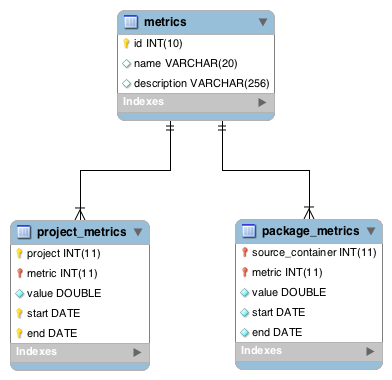
\includegraphics[width=.5\textwidth]{img/dettaglioFinal.png}
	\caption{Nuove relazioni instaurate}\label{fig:dettaglioF}
\end{figure}

Nella fase a priori di impact analysis, gli schemi di \textit{`project\_metrics`} e \textit{`package\_metrics`} erano stati ideati senza i campi per le rispettive start date ed end date. Durante lo sviluppo, si è resa necessaria questa aggiunta avendo incontrato la necessità di prevedere per una stessa metrica valori diversi su archi temporali differenti.\\

C'è da evidenziare come questi cambiamenti, mirati ad adattare la struttura della base di dati alle logiche delle nuove metriche, si siano solamente limitati all'estensione della stuttura relazionale esistente, senza tuttavia richiedere modifiche al comportamento del sistema già sviluppato, il quale potrà continuare a esercitare anche sul database così adattato senza alcuna necessità di intervento supplementare. 

Riportiamo nella figura \ref{fig:repominer} di pagina \pageref{fig:repominer} la struttura del database a seguito delle modifiche effettuatevi, per quanto riguarda le relazioni principali di interesse per il sistema implementato

\begin{figure}[t]
	\centering
	%width=.5\textwidth
	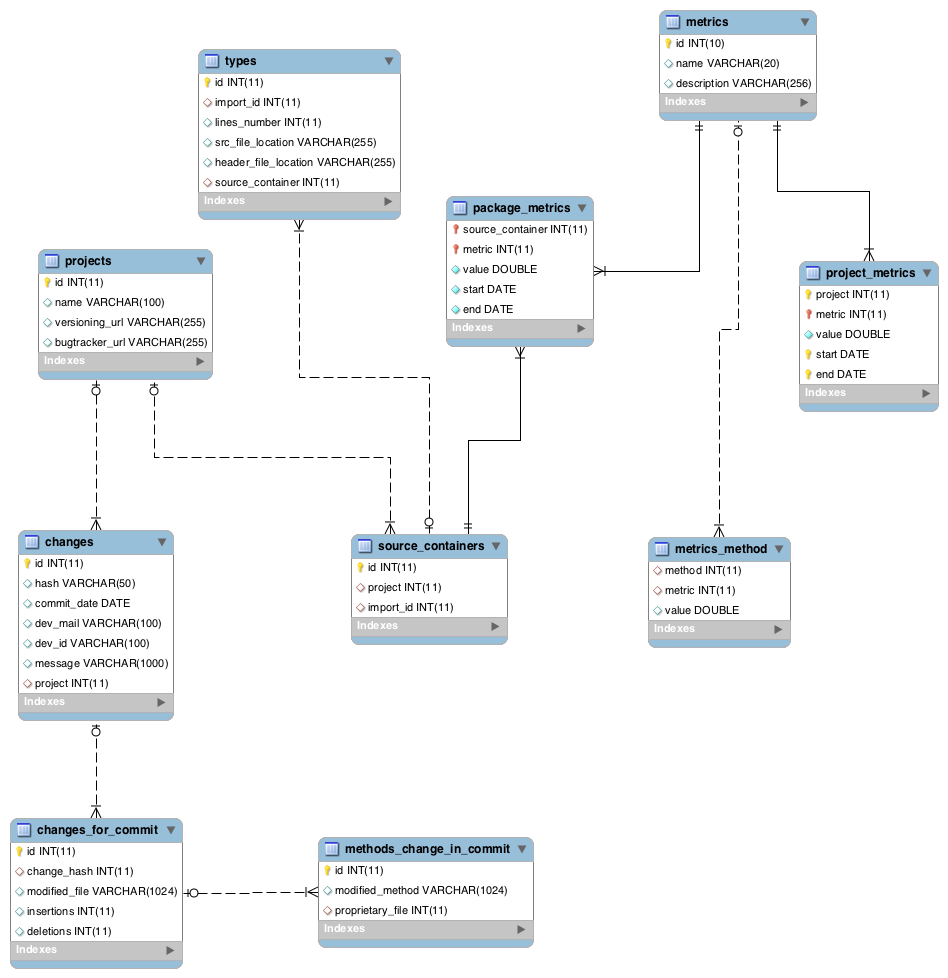
\includegraphics[width=\textwidth]{img/repominer.png}
	\caption{Dettaglio dello schema relazionale modificato}\label{fig:repominer}
\end{figure}
	\chapter{Valutazione del processo}
Per poter valutare l'accuratezza del processo di impacty analysis esistono in letteratura diverse metriche. Nella nostra analisi utilizziamo le due metriche di \textit{recall} e \textit{precision}. Recall misura la parcentuale degli impatti reali inclusi nel Candidate Impact Sect, ossia il seguente rapporto
$$|CIS \cap AIS|\over{|AIS|}$$
La precision invece va a misurare la percentuale di impatti candidati che si sono manifestati come impatti reali. Il rapporto è
$${|CIS \cap AIS|}\over{|CIS|}$$
Fortunatamente, essendo l'impatto sul sistema esistente estremamente limitato e circoscritto solamente alla struttura del database, ci è stato possibile massimizzare entrambe le metriche. Nella fattispecie, il Discovered Impact Set si è rivelato vuoto così come il False Positive Impact Set. Dunque sia la recall che la precision sono pari a 1.

	\chapter{Glossario}
% prova longtable
\begin{center}
\begin{longtable}{lp{.6\columnwidth}}
\hline 
\rowcolor[gray]{.80}
\textbf{Termine} & \textbf{Descrizione} \tabularnewline
\hline 
SIS & 
Starting Impact Set: artefatti che, dopo una analisi delle specifiche della change request, si presume di dover intaccare andando a implementare il cambiamento richiesto
\tabularnewline
\hline
CIS & 
Candidate Impact Set: ulteriore livello di analisi sugli artefatti individuati dal SIS
\tabularnewline
\hline
Recall & 
Metrica per la valutazione del processo di impact analysis che misura la percentuale degli impatti reali inclusi in CIS
\tabularnewline
\hline
Precision & 
Metrica per la valutazione del processo di impact analysis che misura la percentuale degli impatti candidati che sono impatti reali
\tabularnewline
\hline
DIS & 
Discovered Impact Set: sottostima dell'impatto; si tratta degli artefatti che fanno parte dell'AID ma che non sono stati inclusi nel CIS al momento dell'analisi
\tabularnewline
\hline
AID & 
Actual Impact Set: insieme degli artefatti realmente modificati
\tabularnewline
\hline
FPIS & 
False Positive Impact Set: sovrastima dell'impatto; si tratta degli artefatti che sono stati inclusi nel CIS ma che non sono stati impattati
\tabularnewline
\hline
\end{longtable}
\end{center}





	
%\bibliography{bibliografia.bib}{}
%\bibliographystyle{plain}
\end{document}
